% CVPR 2025 Paper Template; see https://github.com/cvpr-org/author-kit

\documentclass[10pt,twocolumn,letterpaper]{article}

%%%%%%%%% PAPER TYPE  - PLEASE UPDATE FOR FINAL VERSION
\usepackage{cvpr}              % To produce the CAMERA-READY version
% \usepackage[review]{cvpr}      % To produce the REVIEW version
% \usepackage[pagenumbers]{cvpr} % To force page numbers, e.g. for an arXiv version

% Import additional packages in the preamble file, before hyperref
%
% --- inline annotations
%
\newcommand{\red}[1]{{\color{red}#1}}
\newcommand{\todo}[1]{{\color{red}#1}}
\newcommand{\TODO}[1]{\textbf{\color{red}[TODO: #1]}}
% --- disable by uncommenting  
% \renewcommand{\TODO}[1]{}
% \renewcommand{\todo}[1]{#1}



% It is strongly recommended to use hyperref, especially for the review version.
% hyperref with option pagebackref eases the reviewers' job.
% Please disable hyperref *only* if you encounter grave issues, 
% e.g. with the file validation for the camera-ready version.
%
% If you comment hyperref and then uncomment it, you should delete *.aux before re-running LaTeX.
% (Or just hit 'q' on the first LaTeX run, let it finish, and you should be clear).
\definecolor{cvprblue}{rgb}{0.21,0.49,0.74}
\usepackage[pagebackref,breaklinks,colorlinks,allcolors=cvprblue]{hyperref}

%%%%%%%%% PAPER ID  - PLEASE UPDATE
\def\paperID{6709} % *** Enter the Paper ID here
\def\confName{CVPR}
\def\confYear{2025}

%%%%%%%%% TITLE - PLEASE UPDATE
\title{\dataset: Learning How Things Move in 3D from Internet Stereo Videos}

%%%%%%%%% AUTHORS - PLEASE UPDATE

\author{
Linyi Jin$^{1,2}$\qquad
Richard Tucker$^1$\qquad
Zhengqi Li$^1$\qquad
David Fouhey$^3$\\
Noah Snavely$^{1*}$\qquad
Aleksander Holynski$^{1*}$
\\[0.5em]
$^1$Google DeepMind \ \ \
$^2$University of Michigan \ \ \ 
$^3$New York University \ \ \ 
$^*$equal contribution\\ \\
}

\begin{document}
\twocolumn[{%
\renewcommand\twocolumn[1][]{#1}%
\maketitle
\vspace{-2em}
 \includegraphics[width=\textwidth]{fig/teaser_v5.pdf}
\captionof{figure}{There is currently no scalable source of data for real-world, ground truth 3D motion paired with video. 
We present a framework for mining such data from existing stereoscopic videos on the Internet, in the form of 3D point clouds with long-range world-space trajectories. Our framework fuses and filters camera poses, dense depth maps, and 2D motion trajectories to produce high-quality, pseudo-metric point clouds with long-term 3D motion trajectories, pictured above, for hundreds of thousands of video clips. We show how this data is useful in learning a model that reasons about both 3D shape and motion in imagery.\\ }
\label{fig:teaser}
}]
\begin{abstract}
Diffusion Models have emerged as powerful generative models for high-quality image synthesis, with many subsequent image editing techniques based on them. However, the ease of text-based image editing introduces significant risks, such as malicious editing for scams or intellectual property infringement. Previous works have attempted to safeguard images from diffusion-based editing by adding imperceptible perturbations. These methods are costly and specifically target prevalent Latent Diffusion Models (LDMs), while Pixel-domain Diffusion Models (PDMs) remain largely unexplored and robust against such attacks. Our work addresses this gap by proposing a novel attacking framework with a feature representation attack loss that exploits vulnerabilities in denoising UNets and a latent optimization strategy to enhance the naturalness of protected images. Extensive experiments demonstrate the effectiveness of our approach in attacking dominant PDM-based editing methods (e.g., SDEdit) while maintaining reasonable protection fidelity and robustness against common defense methods. Additionally, our framework is extensible to LDMs, achieving comparable performance to existing approaches.
\end{abstract}
    
\section{Introduction}
\label{sec:intro}

\begin{figure*}[t]
\centering
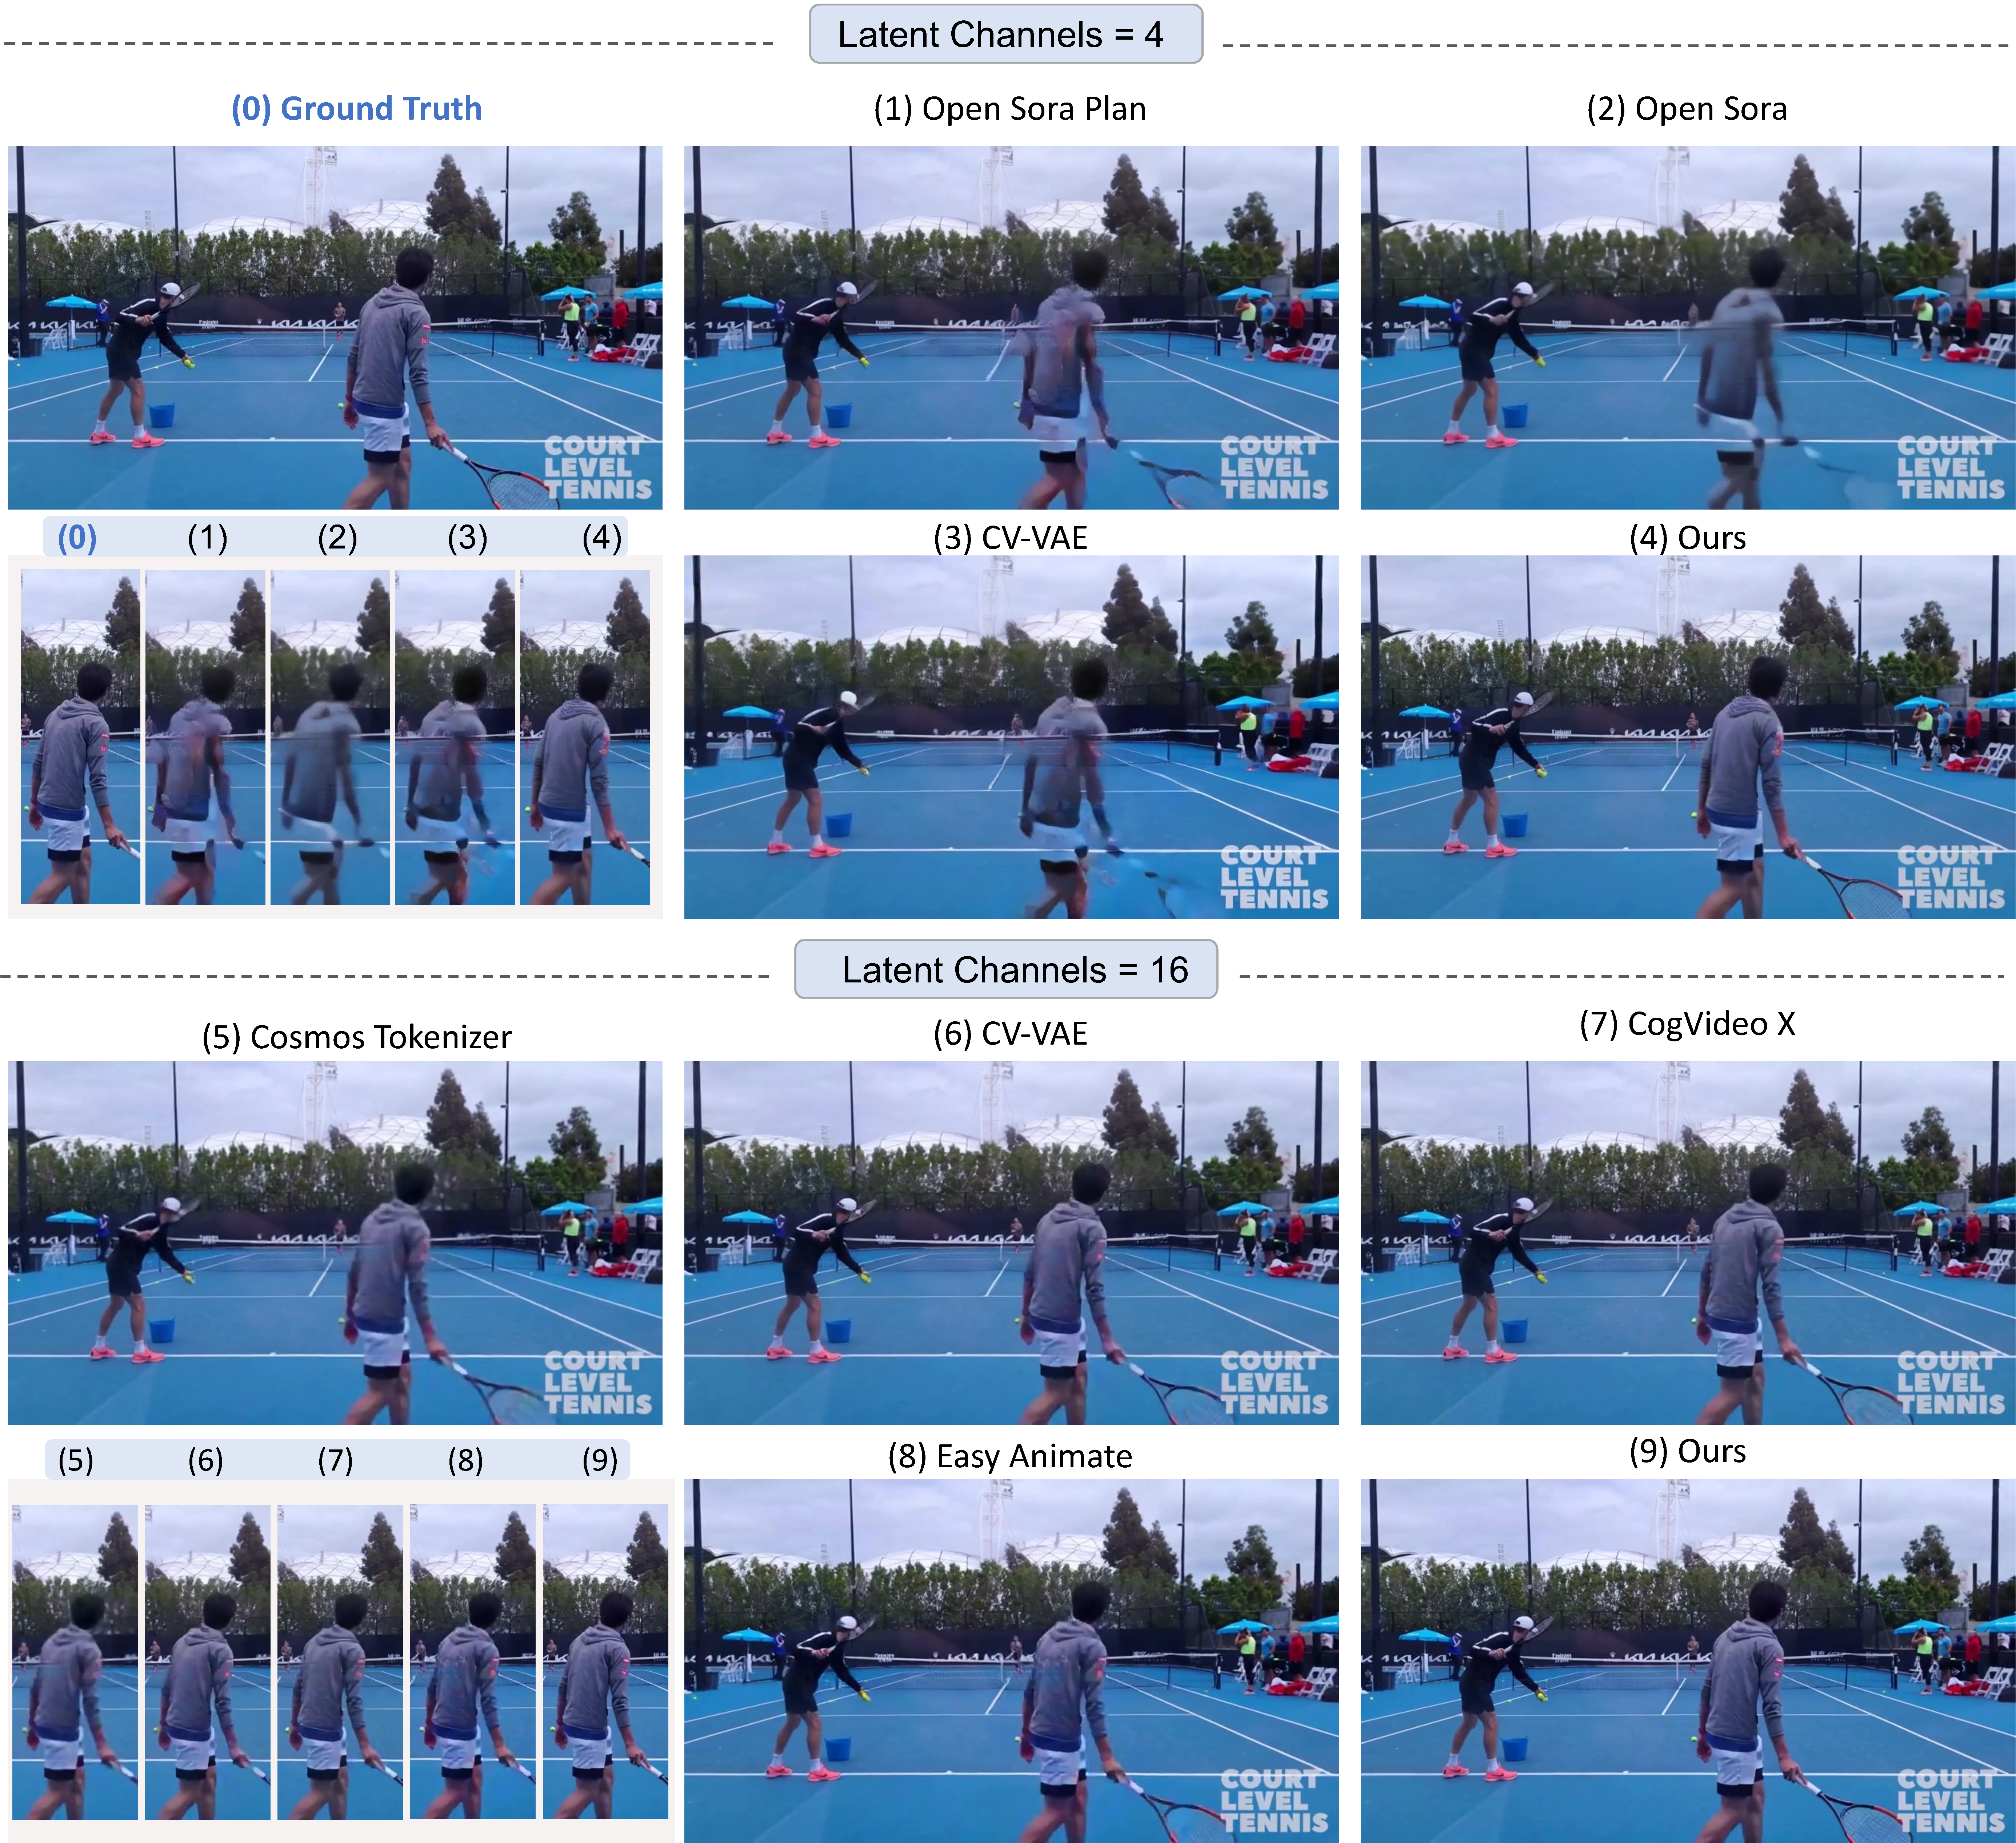
\includegraphics[width=1.0\textwidth]{images/fig1-4and16.pdf}
\caption{
Our reconstruction results compared with a line of three recent strong baseline approaches. 
The ground truth frame is (0). Our model significantly outperforms previous methods, especially under large motion scenarios such as people doing sports.
}
\label{fig:teaser}
\vspace{-3mm}
\end{figure*}



Given the significant attention in the field of video generation, Latent Video Diffusion Models (LVDMs)~\cite{blattmann2023stable, blattmann2023align, he-lvdm, zhou2022magicvideo, he-videocrafter1} have emerged as a popular framework. They have been successfully applied to powerful text-to-video models such as Sora~\cite{videoworldsimulators2024}, VideoCrafter~\cite{he-videocrafter1, chen2024videocrafter2overcomingdatalimitations}, and CogVideoX~\cite{yang2024cogvideox}.
Different from directly generating video pixels, LVDMs generate latent video representations in a compact latent space. This is achieved by first training a Video VAE to encode videos into this latent space.
%
Thus, Video VAE, as a key and fundamental component of LVDMs, has attracted great attention recently.
%
An effective Video VAE can help to reduce the training costs of video diffusion models while improving the final quality of the generated videos.
%
Initially, a series of studies adopt the image VAE from Stable Diffusion~\cite{rombach2022high} for video generation tasks, including AnimateDiff~\cite{guoanimatediff}, MagicVideo~\cite{zhou2022magicvideo}, VideoCrafter1~\cite{he-videocrafter1}, and VideoCrafter2~\cite{chen2024videocrafter2overcomingdatalimitations}. 
%
However, directly adopting an image VAE and compressing video on a frame-by-frame basis leads to temporal flickering due to the lack of temporal correlation. Additionally, the information redundancy along the temporal dimension is not reduced, leading to low training efficiency for subsequent latent video diffusion models.
%
From the introduction of Sora, which compresses videos both temporally and spatially through a Video VAE, a series of studies have emerged that aim to replicate Sora and train their own Video VAEs, including Open Sora~\cite{opensora}, Open Sora Plan~\cite{pku_yuan_lab_and_tuzhan_ai_etc_2024_10948109}, CV-VAE~\cite{zhao2024cv}, CogVideoX~\cite{yang2024cogvideox}, EasyAnimate~\cite{xu2024easyanimatehighperformancelongvideo}, and Cosmos Tokenizer~\cite{cosmos_token}.
%
However, the performance of the current video VAE suffers from many problems, including motion ghost, low-level temporal flickering, blurring (faces, hands, edges, texts), and motion stuttering (lack of correct temporal transition).
% as shown in Fig.~\ref{fig:teaser}.


In this work, we propose a novel cross-modal Video VAE with better spatial and temporal modeling ability in order to solve the aforementioned challenge problems and obtain a robust and high-quality Video VAE.
%
First, we examine different designs for spatial and temporal compression, including simultaneous spatial-temporal (ST) compression and sequential ST compression. 
%
We observed that simultaneous ST compression achieves better low-level temporal smoothness and texture stability, while sequential ST compression achieves better motion recovery, particularly in scenarios of large motion.
%
Thus, we propose a novel architecture that integrates the advantages of both methods and enables effective video detail and motion reconstruction.

Second, we observed that the normally used datasets for text-to-video generation contain text-video pairs. 
Also, during decoding, a text description exists as it serves as the input in the first stage, \textit{i.e.}, the video latent generation stage.
%
To this end, we integrate the text information into the encoding and decoding procedure and propose the first Cross-modal Video VAE.
%
We carefully study how text guidance can be integrated into the spatiotemporal backbone and the mechanism of spatial and temporal semantic guidance. 

In addition, our cross-modal video VAE supports image-video joint training.
To achieve this, we design our network with a fully spatiotemporal factorized architecture, and we feed image and video batches alternately to the network. 
%
During image batches, the data only forwards the spatial part of the network, with the temporal modules being skipped. During video batches, the video forwards both spatial and temporal modules. We also demonstrate that image joint training is crucial for training a video VAE.
%
In summary, our contributions are as follows:
\begin{itemize}
    \item We propose an effective and robust Video VAE, conduct extensive experiments, and achieve the state-of-the-art.
    \item We propose an optimal spatiotemporal modeling approach for Video VAE.
    \item We propose the first cross-modal video VAE that leverages the information from other modalities, i.e., text descriptions, to the best of our knowledge.
    \item Our video VAE is designed and trained to be versatile to conduct both image and video compression. 
\end{itemize}


% \vspace{-2mm}
\section{Related Work}
% \vspace{-2mm}
\label{sec:formatting}
%We now review relevant works on segmentation, vision transformers, and efficient attention.

%-------------------------------------------------------------------------
% \subsection{Video Object Segmentation}
{\bf Video Object Segmentation (VOS)} is a fundamental task in computer vision, segments objects of interest from the background and tracks target objects in a video. 
%Many research works have been proposed in this community on video object segmentation. 
In the unsupervised setting~\citep{grundmann2010efficient,brox2010object,lee2011key,xu2012evaluation,fragkiadaki2012video,perazzi2012saliency,zhang2013video,li2013video,papazoglou2013fast,faktor2014video,wang2015saliency,taylor2015causal,perazzi2016benchmark}, VOS models segment salient objects without a reference mask. In the semi-supervised setting~\citep{pont20172017,xu2018youtube,oh2019video,bhat2020learning,robinson2020learning,li2022recurrent,yang2022decoupling,cheng2022xmem,zhang2023joint,wang2023look,wu2023scalable,cheng2024putting,yang2024scalable}, VOS requires tracking and segmenting objects based on a first-frame mask of target objects. For interactive video object segmentation (iVOS)~\citep{caelles20182018,heo2020interactive,cheng2021modular,homayounfar2021videoclick,yang2023track,cheng2023segment,rajivc2023segment,cheng2024putting,delatolas2024learning}, iVOS models perform object segmentation in videos (masklets) with user guidance, e.g., clicks, bounding boxes, scribbles. In SAM 2~\citep{ravi2024sam}. Semi-supervised VOS and iVOS have been extended to promptable visual segmentation (PVS), where the model can be interactively prompted with different types of inputs such as clicks, boxes, and masks on any frame in a video for segmenting and tracking a valid object.
%-------------------------------------------------------------------------

% \subsection{Vision Transformers}
\noindent {\bf Vision Transformers (ViTs)} have achieved huge success on various vision tasks including image classification~\citep{dosovitskiy2020image}, object detection~\citep{li2022exploring}, image segmentation~\cite{cheng2022masked,kirillov2023segment}, video classification~\citep{fan2021multiscale}, and video object segmentation~\citep{duke2021sstvos,yang2023track}. The original ViT family scales from the efficient ViT-Tiny up to ViT-Huge, with a plain, non-hierarchical architecture. There are also hierarchical vision transformers that combine transformers with hierarchical stage structure, such as Swin~\citep{liu2021swin}, MViT~\citep{fan2021multiscale,li2022mvitv2}, PViT~\citep{wang2021pyramid}, and Hiera~\citep{ryali2023hiera}. While being successful, hierarchical models are usually slower than their plain ViT counterparts for practical deployment~\citep{ryali2023hiera}. 
Combining ViT with convolutions~\citep{lecun1989backpropagation} has been explored for fast hybrid models such as MobileViT~\citep{mehta2021mobilevit}, LeViT~\citep{graham2021levit},  EfficientFormer\citep{li2022efficientformer}, Next-ViT\citep{li2022next}, Tiny-ViT\citep{wu2022tinyvit}, Castling-ViT\citep{you2023castling}, EfficientViT~\citep{liu2023efficientvit}, and MobileNetv4~\citep{qin2024mobilenetv4}. This line of progression towards building efficient ViTs is orthogonal to our
EfficientTAM work towards building efficient video object segmentation. Following SAM~\citep{kirillov2023segment} and EfficientSAMs~\citep{xiong2024efficientsam}, we are pursuing plain ViT backbones for efficient video object segmentation and track anything tasks.  
%The community has also shown increasing interest in efficient vision transformers; \citep{touvron2021training} presented smaller ViTs such as ViT-Small and ViT-Tiny for complementing ViT-Huge, ViT-Large, and ViT-Base in \citep{dosovitskiy2020image}. 


%-------------------------------------------------------------------------
% \subsection{Efficient Attention}
\noindent {\bf Efficient Attention.} The field has developed methods to reduce the quadratic cost of standard self-attention with respect to input sequence length~\cite{attention_is_all_you_need}. 
Local windowed attention has been applied in \cite{beltagy2020longformer,zaheer2020bigbird} for reducing the complexity of self-attention. In \cite{shen2018efficient,katharopoulos-et-al-2020}, a linear dot product approximation is proposed to linearize the softmax matrix in self-attention by heuristically separating keys and queries. In \cite{choromanski2020rethinking}, the Performer model uses random features to approximate self-attention, achieving linear time and memory cost. Nystr\"{o}mformer in \cite{xiong2021nystromformer} makes use of the Nystr\"{o}m method to approximate self-attention with a linear cost. Linformer \cite{wang2020linformer} shows that self-attention is low-rank, which can be approximated by learning linear projection matrices for the keys and values. The approach of~\citep{liu2023efficientvit,you2023castling} leverages the associative property of matrix multiplication for efficient attentions in vision transformers. This direction has shown success and has achieved decent performance on vision tasks. However, in preliminary experiments we found that these methods underperformed in a memory cross-attention module when adapted for efficiency improvement.


%-------------------------------------------------------------------------
% \subsection{Segment Anything Model}
\noindent {\bf Segment Anything Model.} SAM~\citep{kirillov2023segment} is a vision foundation model that can segment any object in an image using interactive prompts such as points and bounding boxes. SAM has demonstrated remarkable zero-shot transfer performance and high versatility for many vision tasks including a broad range of segmentation applications~\citep{chen2023semantic,cen2023sad,deng2023segment,chen2023sam}, in-painting~\citep{yu2023inpaint}, image restoration~\citep{jiang2023restore}, image editing~\citep{gao2023editanything}, image shadow removal~\citep{zhang2023deshadow}, medical image segmentation~\citep{ma2023segment}, camouflaged object detection~\citep{tang2023can}, transparent object detection~\citep{han2023segment}, concept-based explanation~\citep{sun2023explain}, semantic communication~\citep{tariq2023segment}, and object tracking~\citep{cheng2023segment,yang2023track}. The strong ability on image segmentation with flexible prompts motivates the extension of SAM for video object segmentation and track anything. Track Anything Model (TAM)~\citep{yang2023track} combines SAM and XMem~\cite{cheng2022xmem} for interactive video object tracking and segmentation with SAM for frame segmentation and XMem for tracking. SAM-Track~\citep{cheng2023segment} perform object tracking and segmentation in videos by combining SAM~\citep{kirillov2023segment}, DeAOT~\citep{yang2022decoupling}, and Grounding-Dino~\citep{liu2023grounding}. The latest SAM 2~\citep{ravi2024sam} extended SAM for video segmentation through a hierarchical image encoder for frame embeddings and a memory module that conditions current frame embeddings on past frames. Motivated by mobile app use-cases and computationally-constrained applications, recent works have reduced the computational cost of SAM, such as MobileSAM~\citep{zhang2023faster}, FastSAM~\citep{zhao2023fast}, and EfficientSAM~\citep{xiong2024efficientsam}.
The present paper focuses on improving the efficiency challenges of SAM 2 for practical deployment of video object segmentation and track anything.  

\section{Creating a dataset of 4D scenes}
\label{sec:data}


\begin{figure}
    \centering
    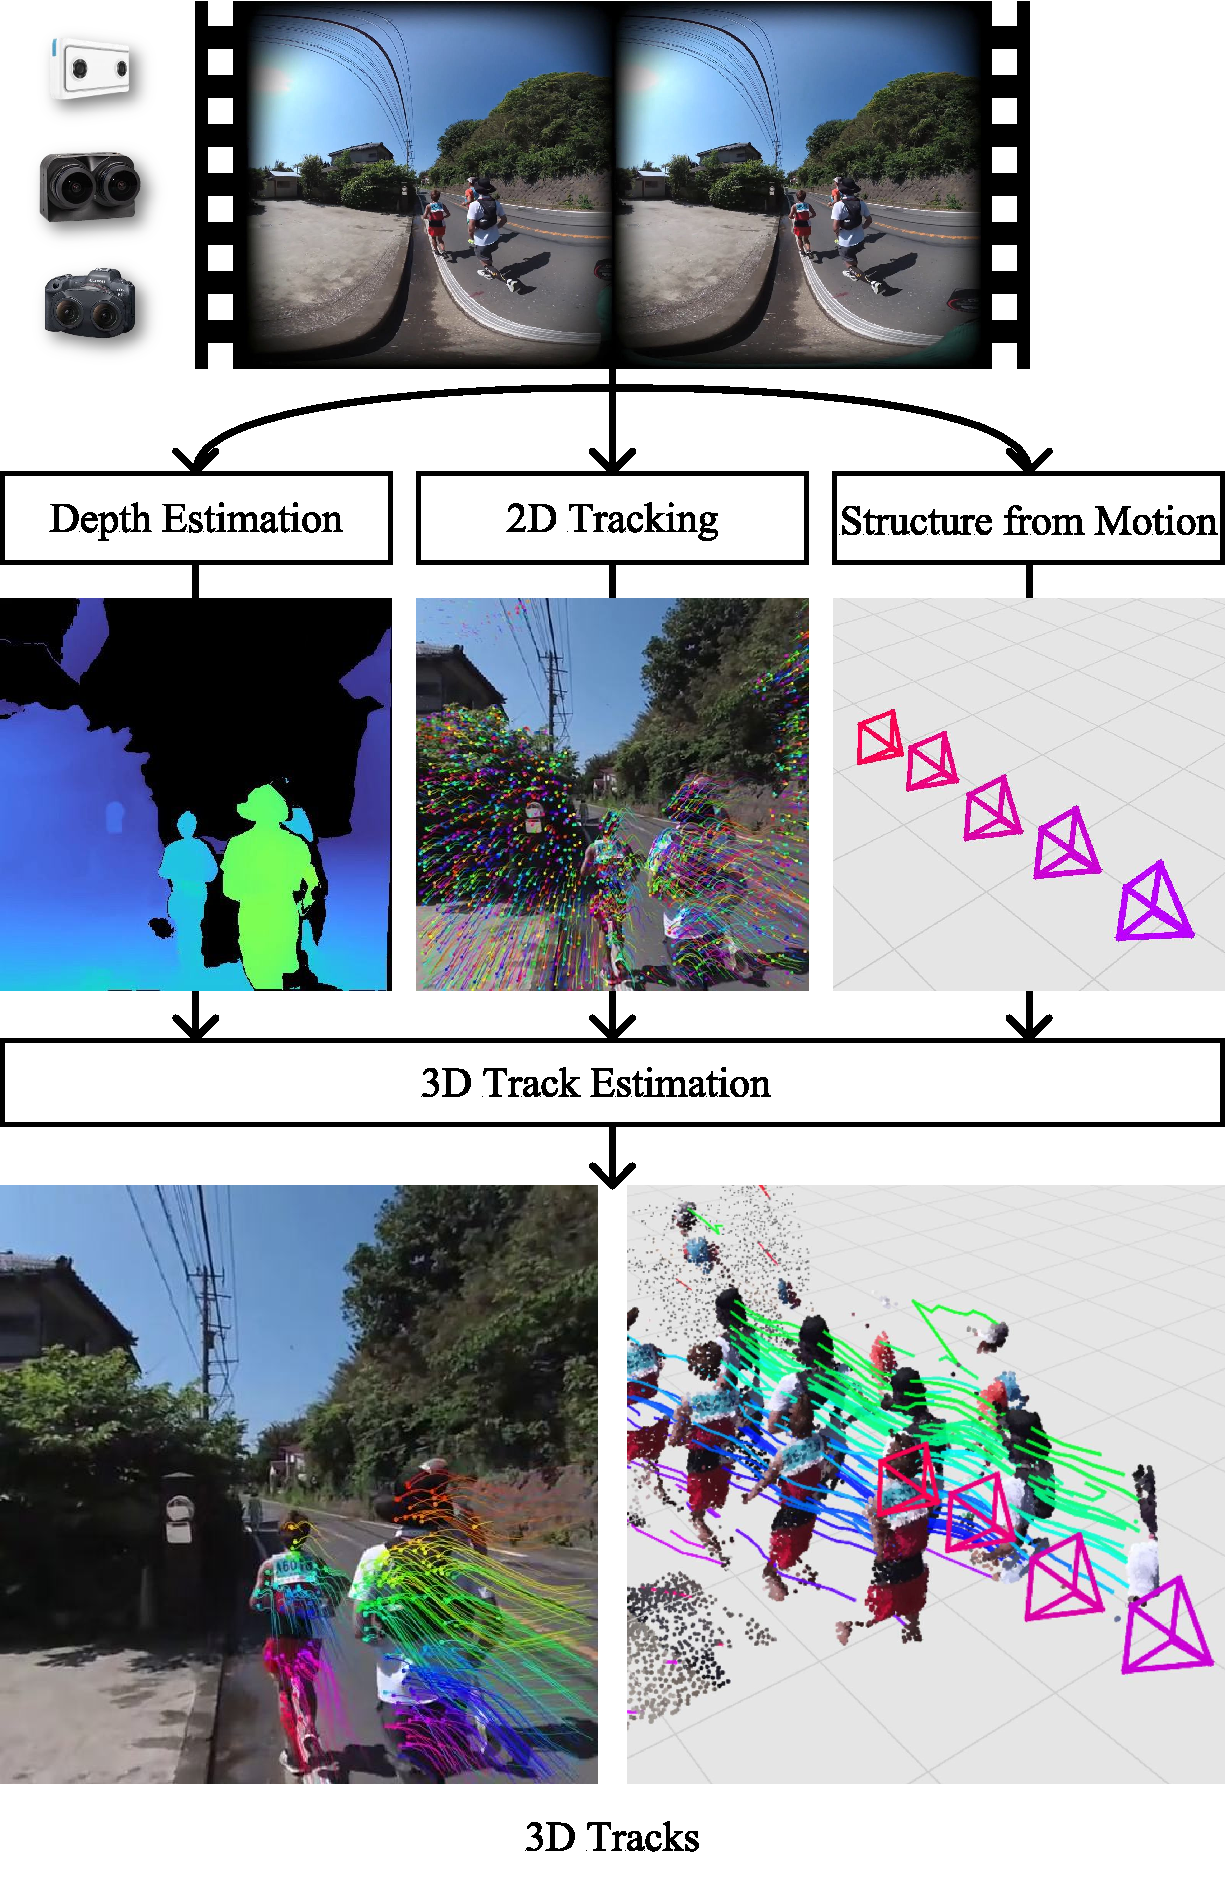
\includegraphics[width=\linewidth]{fig/data_processing_vertical.pdf}
    \vspace{-2em}
    \caption{\textbf{Data processing pipeline.} Our method starts with VR180 (wide-angle, stereoscopic) videos, and estimates metric stereo depth, 2D point tracks, and camera poses. These quantities allow the tracks to be lifted to 3D where they are filtered and denoised to produce world-space, metric 3D point trajectories.}
    \label{fig:data_pipeline}
\end{figure}

A core contribution of this work is a pipeline for extracting high-quality, pseudo-metric, 3D data from online stereoscopic fisheye videos (known as VR180 videos). 
High-resolution, wide field of view VR180 videos can be found readily online.
We show that this data is ideal for deriving rich dynamic 3D information that can power models for predicting geometry and motion from imagery.

Concretely, each instance of data starts as an $N$ frame stereo video consisting of left-right image pairs $\IB_i$ and $\IB'_i$ indexed by frame index $i\in[1,N]$. We convert these stereo pairs to a dynamic 3D point cloud with $K$ points in a world-space coordinate frame, where each point, indexed by $j\in[1,K]$, has a time-varying position $\pB_i^j$. 
As part of the process of generating this dynamic point cloud, we also extract a number of auxiliary quantities: (1) per-frame camera extrinsics, (the left camera's position $\cB_i$ and orientation $\RB_i$), (2) rig calibration for the stereo video giving the position $\cB_r$ and orientation $\RB_r$ of the right camera relative to the left camera, and (3) a per-frame disparity map $\DB_i$.


\subsection{Data Processing Pipeline} 

At a high level, our pipeline for converting a stereoscopic video into a dynamic point cloud involves estimating camera poses, stereo disparity, and 2D tracks, fusing these quantities into a consistent 3D coordinate frame, and performing several filtering operations to ensure temporal consistent, high-quality reconstructions (\Fig{data_pipeline}). In this section, we describe in detail the key components of this process. %


\medskip
\noindent \textbf{SfM.} 
We start by processing the sequence of stereo frames $\IB_i \leftrightarrow \IB_i'$ to produce camera pose estimates ($\cB_i, \RB_i$). We first use a SLAM method to divide the video into shots, as in~\cite{zhou2017scene}. For each shot, we run an incremental SfM algorithm similar to COLMAP~\cite{schonberger2016structure}. We initialize the stereo rig calibration $(\cB_r, \RB_r)$ to a rectified stereo pair with baseline $6.3$cm, but optimize for the calibration in bundle adjustment. In practice, we found that the exact stereo pair orientation can vary significantly from its nominal configuration and that optimizing the rig was critical for good results. 

\medskip 
\noindent \textbf{Depth Estimation.}
We next estimate a per-frame disparity map, operating on each frame independently. In particular, we use the estimated camera rig calibration $\cB_r, \RB_r$ to create rectified stereo pairs from the stereo fisheye video and estimate the per-frame disparity~$\DB_i$ with RAFT~\cite{sun2022disentangling,
sun2021autoflow,teed2020raft}. 

\medskip
\noindent \textbf{3D Track Estimation and Optimization.}  %
We extract long-range 2D point trajectories using BootsTAP~\cite{doersch2024bootstap}. Using the camera poses $\cB_i, \RB_i$ and disparity maps $\DB_i$, we unproject these tracked points into 3D space, turning each 2D track $j$ into a 3D motion trajectory $\pB^j_1, \ldots, \pB^j_N$
 across all frames. In general, each point will usually only be tracked in a subset of frames, but for simplicity, we describe the formulation as if all points are always visible. Moreover, since subsequent steps are done independently per-track, we drop the superscript $j$ in future references. 

Since stereo depth estimation is performed per-frame, the initial disparity estimates (and therefore, the 3D track positions) are likely to exhibit high-frequency temporal jitter. To compensate for potentially inconsistent disparity estimates, we formulate an optimization strategy that solves for a per-frame scalar offset $\delta_i \in \mathbb{R}$ that moves each point $\pB_i$ along the ray from camera location $\cB_i$ to $\pB_i$ at frame $i$. 
This ray is denoted $\rB_i = (\pB_i - \cB_i) / ||\pB_i - \cB_i||$, and we refer to the updated location as $\pB_i' = \pB_i + \delta_i \rB_i$. 

To ensure static points remain stationary while moving tracks maintain realistic, smooth motion, avoiding abrupt depth changes frame by frame, we design an optimization objective comprising three terms: a static loss $\mathcal{L}_{\mathsf{static}}$, a dynamic loss $\mathcal{L}_{\mathsf{dynamic}}$, and a regularization loss $\mathcal{L}_{\mathsf{reg}}$. The static loss $\mathcal{L}_{\mathsf{static}}$ minimizes jitter by encouraging points to remain close to each other in world space:
\begin{equation}
\mathcal{L}_{\mathsf{static}} = \sum_{i=1}^{N} \sum_{j=1}^{N} \frac{\| \mathbf{p}_i' - \mathbf{p}_j' \|^2}{N_p'^2}
\label{eq:objective_function}
\end{equation}
where $N_p' = \sum_{i=1}^N{\|\mathbf{p}'_i\|} / N$ is a normalizing factor.
The dynamic loss term reduces jitter by minimizing acceleration along the camera ray through a discrete Laplacian operator:
\begin{equation}
\mathcal{L}_{\mathsf{dynamic}} = \sum_{i=1}^{N} \sum_{\Delta\in\mathcal{W}} \left[ \left( \mathbf{p}_{i+\Delta}' - 2\mathbf{p}_i' + \mathbf{p}_{i-\Delta}' \right)^\top \mathbf{r}_i \right]^2
\label{eq:dynamic_objective}
\end{equation}
where the acceleration along the ray is calculated over
multiple window sizes $\mathcal{W}=\{1,3,5\}$.


The two loss terms are weighted by a track-dependent function, $\sigma(m)$, where $m$ is a measure of the motion magnitude of the track. Motion is measured in 2D rather than 3D because distant points can appear to have a larger 3D motion due to noise amplification at low disparities.
Specifically, we project the 3D motion trajectory between time $i - w_o$ and the current time $i$ into 2D image-space at time $i$, %
and calculate the track's motion magnitude $m$ as the 90$^{th}$ percentile of the track's trail length across all frames. The track trail length for a frame is measured by projected 3D points along the track to the current frame as if the camera is \emph{static} in a window of $w_o=16$ frames, 
\begin{equation}
\label{eqn:trail_length_def}
    m = \mathsf{Percentile}_{i=1:N}^{90}\left[\max_{w=1:w_o}\|\pi_i(\pB_i) - \pi_i(\pB_{i-w})\|\right]
\end{equation}
where $\pi_i(\cdot)\in \mathbb{R}^2$ gives the projected pixel location of a 3D point on camera $\cB_i$'s image plane.
The weighting function $\sigma(m)$ is defined as $\sigma(m) = \frac{1}{1 + \exp(m - m_0)}$ where $m_0 = 20$. 
Finally, to encourage faithfulness to the originally estimated disparities, we regularize the displacements in disparity space:
\begin{equation}
    \mathcal{L}_{\mathsf{reg}} = \lambda_{\mathsf{reg}} \sum_{i=1}^{T} \left( \frac{1}{\delta_i + \|\mathbf{p}_i-\mathbf{c}_i\|} - \frac{1}{\|\mathbf{p}_i-\mathbf{c}_i\|} \right)^2,
\end{equation}
where use of disparity space reflects the fact that the measurements themselves originate as disparities. Practically, the impact of the use of disparity is that larger deviations are tolerated at more distant points, where depth is intrinsically more uncertain.

The full objective function is
\begin{equation}
\min_{\{\delta_i\}_{i=1}^N} \sigma(m)\mathcal{L}_{\mathsf{static}} + (1-\sigma(m))\mathcal{L}_{\mathsf{dynamic}} + \mathcal{L}_{\mathsf{reg}}.
\label{eqn:objective}
\end{equation}
We set $\lambda_{\mathsf{reg}}=10^{-4}$ and optimize Eqn.~\ref{eqn:objective} using Adam with a learning rate of 0.05 for 100 steps.
The effect of track optimization is shown in \Fig{track_optimization}. The optimized motion is smoother and does not contain high frequency noise.


\begin{figure}[t]
    \centering
    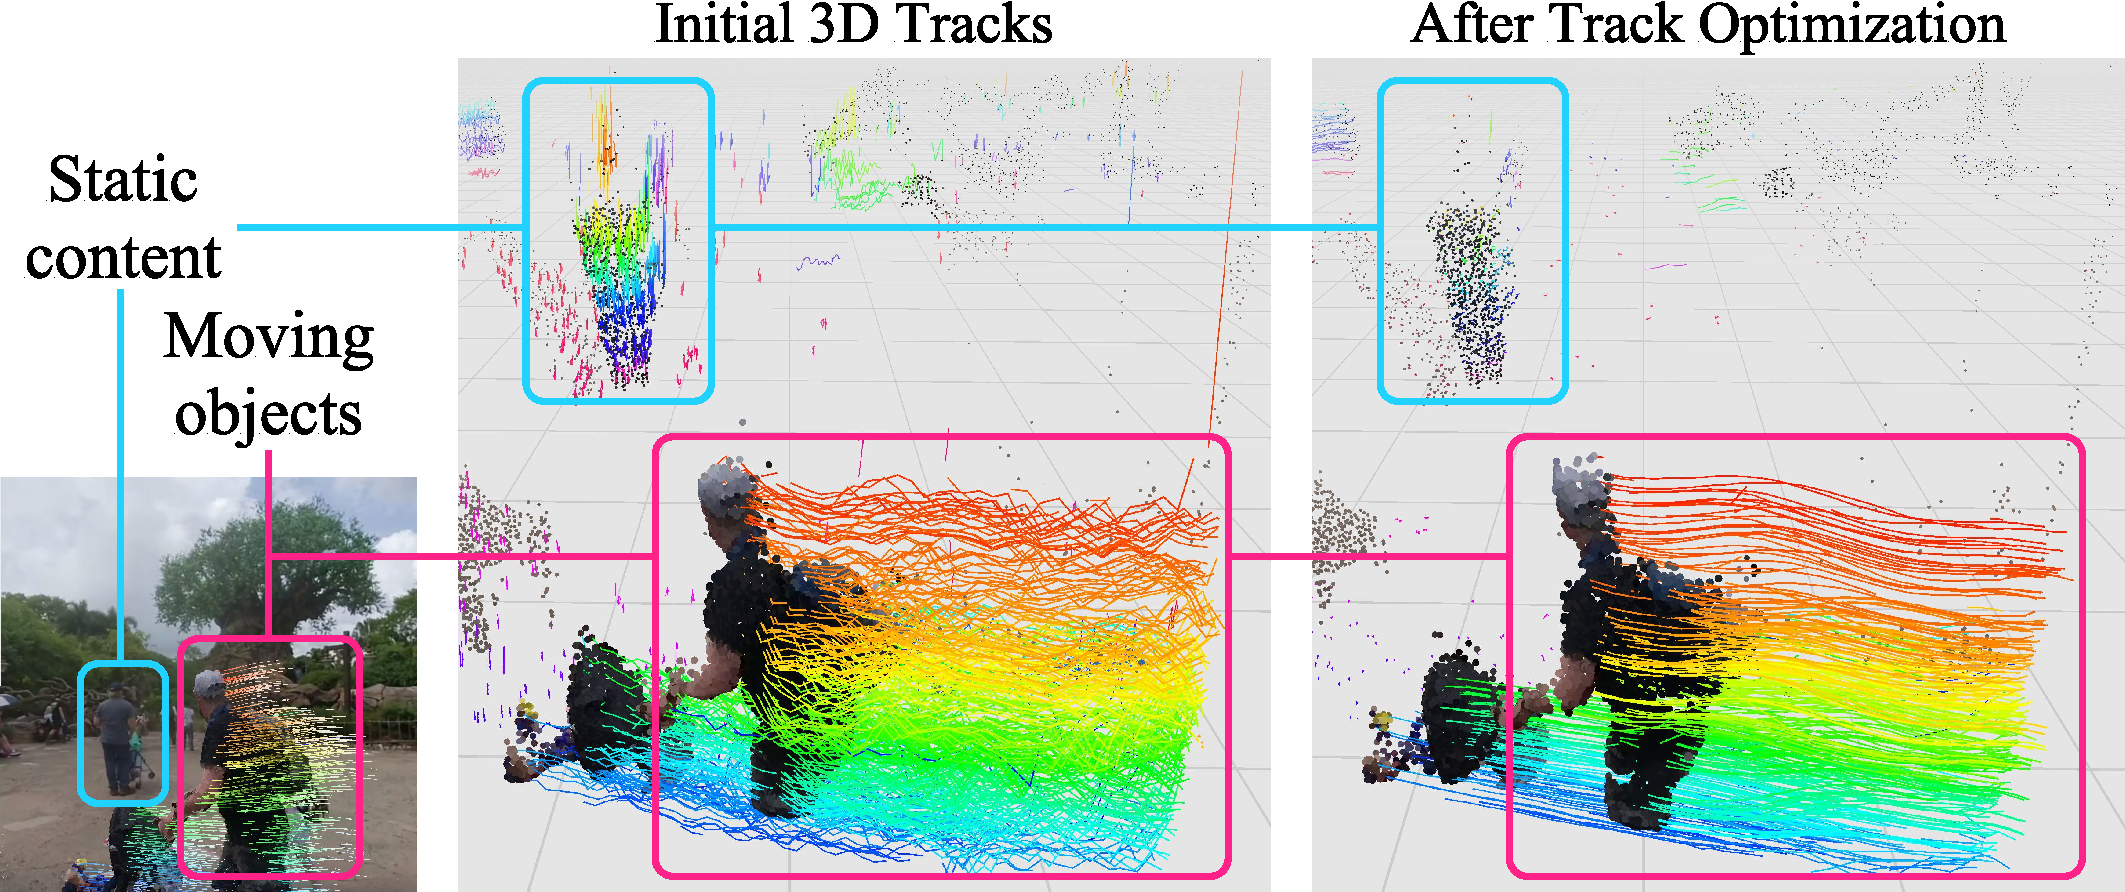
\includegraphics[width=\linewidth]{fig/optimization.pdf}
    \caption{\textbf{Effect of track optimization.} Comparing motion trajectories before and after track optimization, we see that optimization resolves the high frequency jitter along camera rays, affecting both static and dynamic content. After optimization, static content has static tracks, and dynamic tracks are less noisy.}
    \label{fig:track_optimization}
\end{figure}


\begin{figure*}[t]
\vspace{-1em}
    \centering
    \includegraphics[width=\textwidth]{fig/diversity-highres.pdf}
    \caption{\textbf{Diverse motion:} \dataset captures a wide variety of types of moving objects, from swimming fish, to walking pedestrians, moving vehicles, and a farmer sowing seeds. It includes source videos captured with both stationary (left) and moving (right) cameras.}
    \label{fig:motion_distribution}
\end{figure*}
\medskip
\noindent \textbf{Implementation details.} %
{\it Shot-selection.} Rather than work with the full video, we break the footage into discrete, trackable shots using ORB-SLAM2's stereo estimation mode~\cite{murartal2015orbslam} following~\cite{zhou2018stereo}. 
{\it Field of View.} While estimating pose, we use a $140^\circ$ FoV fisheye format, which we found to capture more of the (usually static) background and less of the (often dynamic) foreground, yielding more reliable camera poses. 
{\it Stereo Confidence Checks.} We discard pixels where the $y$-component of RAFT flow is more than 1 pixel (since rectified stereo pairs should have perfectly horizontal motion) and where the stereo cycle consistency error is more than 1 pixel (since such pixels are unreliable). 
{\it Dense 2D tracks.} To get dense tracks, we run BootsTAP with dense query points: for every 10th frame, we uniformly initialize $128\times128$ query points on frames of resolution 512 $\times$ 512. We then prune redundant tracks that overlap on the same pixel.
{\it Drifting tracks.} Since 2D tracks can drift on textureless regions, we discard moving 3D tracks that correspond to certain semantic categories (\textit{e.g.}, ``walls'', ``building'', ``road'', ``earth'', ``sidewalk''), detected by DeepLabv3~\cite{chen2017rethinking} on ADE20K classes~\cite{zhou2017scene, zhou2019semantic}.

\medskip
\noindent \textbf{Filtering details.} A fraction of the video clips that are processed may be unsuitable because they either (1) are not videos, and are entirely static images, (2) contain cross-fades, or (3) have text or other synthetic graphics. To discard text and title sequences, we avoid creating video clips from the start and ends of the source videos. We identify cross-fades by running SIFT~\cite{lowe2004sift} matching through the video at multiple temporal scales and discarding video clips with static camera but with fewer than 5 SIFT matches between frames that are 5 seconds apart.



\begin{figure}[t]
    \centering
    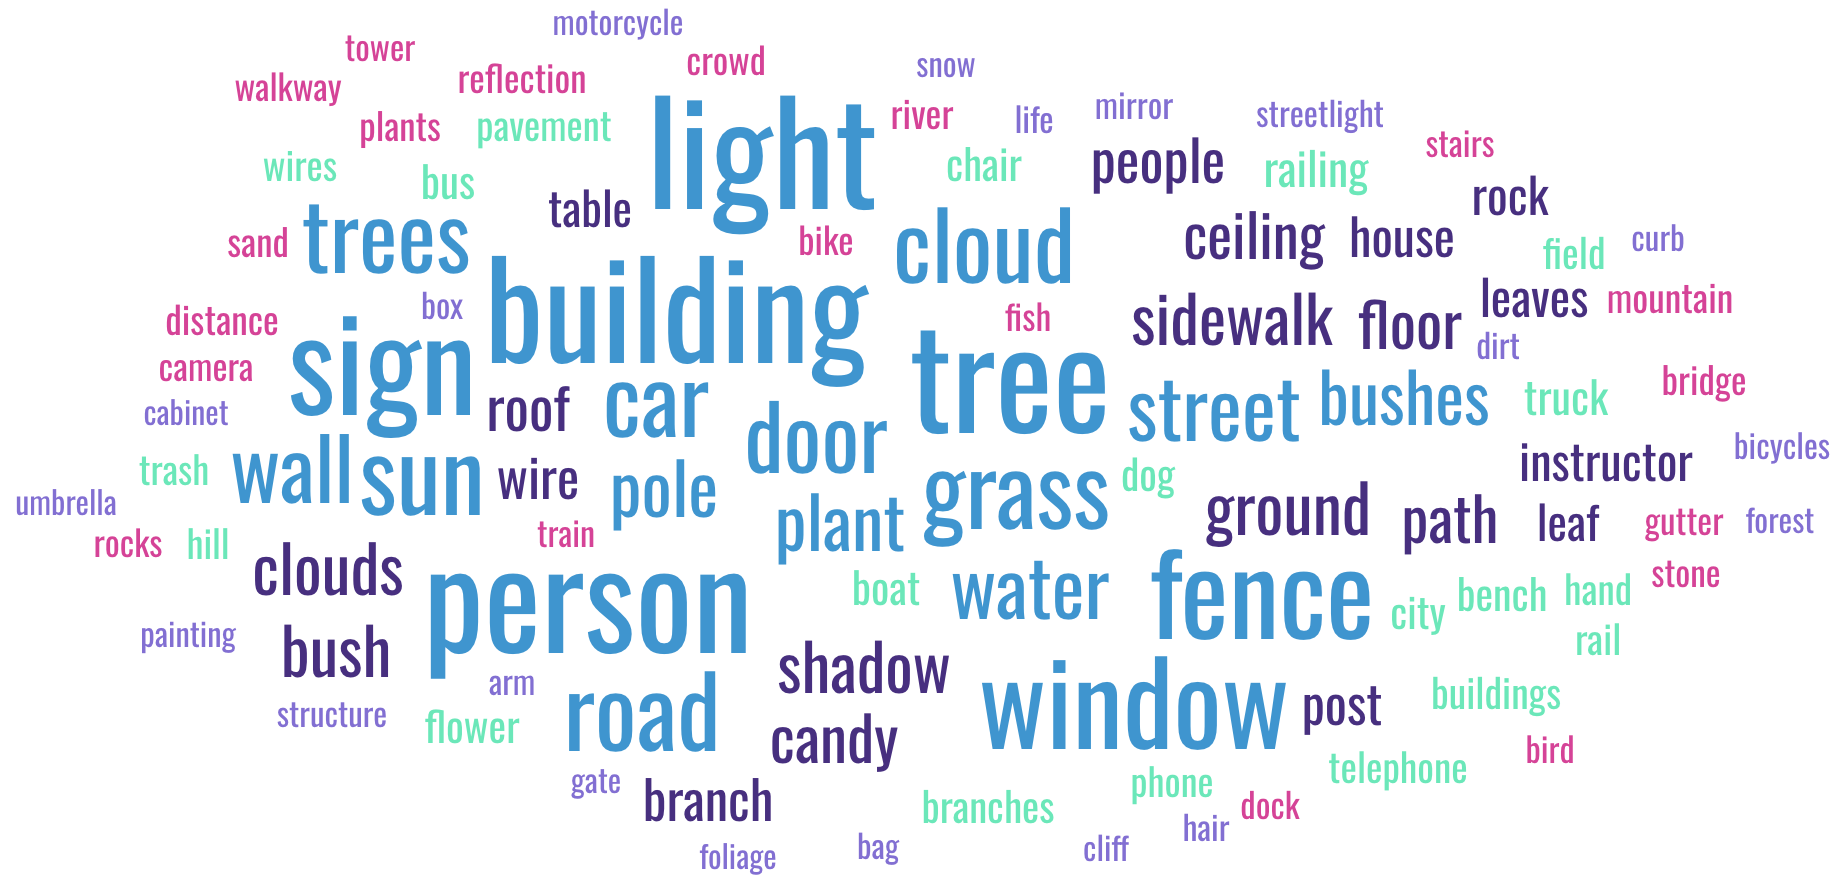
\includegraphics[width=\linewidth]{fig/wordcloud.png}
    \caption{\textbf{Diverse scene content:} A word cloud of captioned frames from our dataset shows our data is diverse, including a variety of common objects seen in videos.}
    \label{fig:wordcloud}
\end{figure}


\subsection{Stereo4D Dataset}

\Fig{motion_distribution} illustrates a subset of videos and reconstructions from a dataset processed with the above pipeline, encompassing more than 100K clips capturing everyday scenes and activities. To visualize the range of content, we used an automatic captioning system to generate captions for the dataset and created a word cloud (\Fig{wordcloud}) highlighting the most frequently observed objects.






\begin{figure}[t]
    \centering
    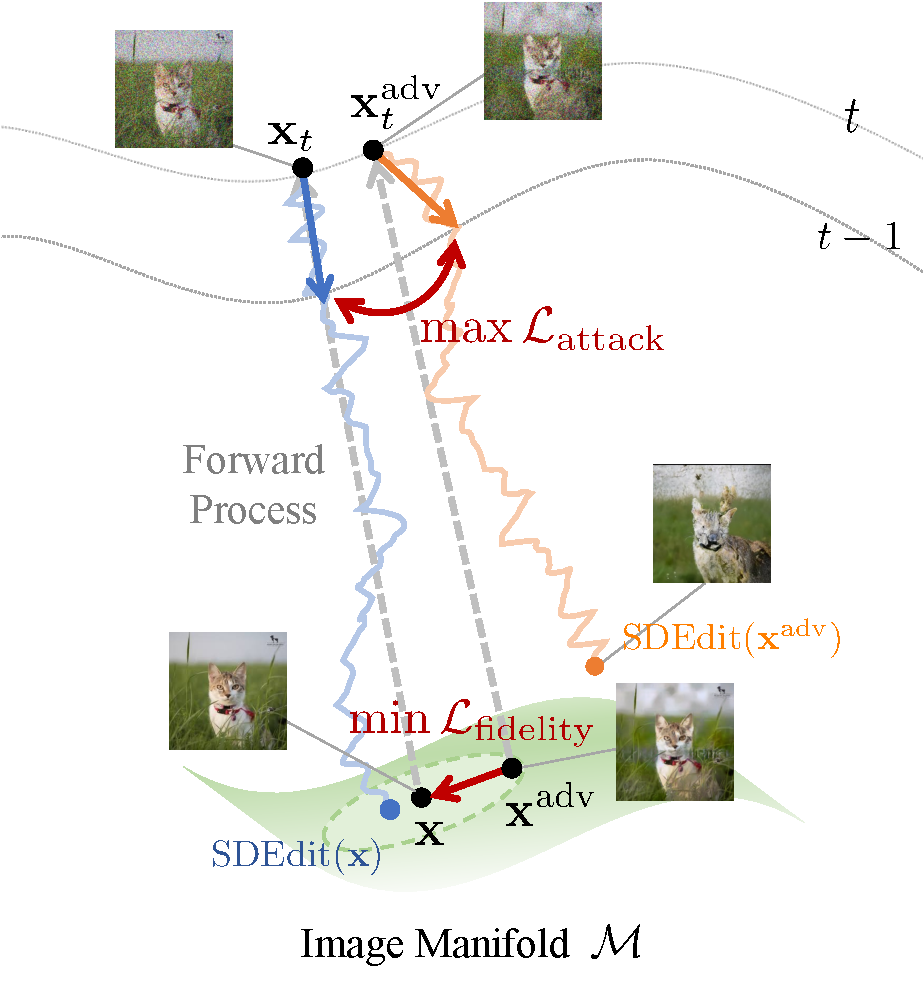
\includegraphics[width=1\linewidth]{figures/manifold.pdf}
    \caption{Conceptual illustration of our method. We randomly forward both the clean image $\mathbf{x}$ and adversarial image $\mathbf{x}^{\adv}$ to noise level $t$, then utilize our feature attacking loss to maximize the feature distance between noisy latent $\mathbf{x}_t$ and $\mathbf{x}^{\adv}_t$ in the reverse process of diffusion models while imposing our fidelity loss as a constraint to ensure the adversarial image from being deviated from the original image. We update the $\mathbf{x}^{\adv}$ in latent space instead of in pixel space to ensure the naturalness of $\mathbf{x}^{\adv}$.}
    \label{concept}
\end{figure}


\section{Methodology}

\subsection{Threat Model and Problem Setting}
The malicious user collects an image $\mathbf{x}$ from the internet and uses SDEdit \cite{meng2021sdedit} to generate unauthorized image translations or editing, denoted as $\text{SDEdit}(\mathbf{x}, t)$, that manipulates the original input image $\mathbf{x}$.

Our work aims to safeguard the input image $\mathbf{x}$ from the authorized manipulations by crafting an adversarial image $\mathbf{x}^{\adv}$ by adding imperceptible perturbation to disrupt the reverse diffusion process of SDEdit for corrupted editions.

For example, we want the main object of the image, e.g., the cat in the source image $\mathbf{x}$ as shown in Figure~\ref{concept} unable to be reconstructed by the reverse diffusion process. Meanwhile, the adversarial image should maintain similarity to the source image to ensure fidelity. The reason why we target SDEdit as our threat model is that it is recognized as the most common and general operation in diffusion-based unconditional image translations and conditional image editing. Additionally, it has been incorporated into various editing pipelines~\cite{tsaban2023leditsrealimageediting, zhang2023inversion}. Here we focus on the unconditional image translations for our main study, as they are essential in both unconditional and conditional editing pipelines. Formally, our objective to effectively safeguard images while maintaining fidelity is formulated as:

\begin{equation}
    \begin{aligned}
        & \max_{\mathbf{x}^{\adv} \in \mathcal{M}} d(\text{SDEdit}(\mathbf{x}, t), \text{SDEdit}(\mathbf{x}^{\adv}, t)) \\
    & \text{subject to } d^{\prime}(\mathbf{x}, \mathbf{x}^{\adv}) \leq \delta,
    \end{aligned}
    \label{eq:probelm_setting_constraint}
\end{equation}

where $\mathcal{M}$ indicates natural image manifold, $d$, $d^{\prime}$ indicate image distance functions and $\epsilon$ denotes the fidelity budget.

In the following sections, we first present a conceptual illustration of our method, followed by our framework for solving the optimization problem. We then discuss the novel design of our attacking loss and fidelity constraints, which provide more efficient criteria compared to previous methods for solving the image protection optimization problem using PGD. Finally, we introduce an advanced design to enhance image protection quality by latent optimization via victim-model-agnostic VAE.

\begin{figure*}[t]
    \centering
    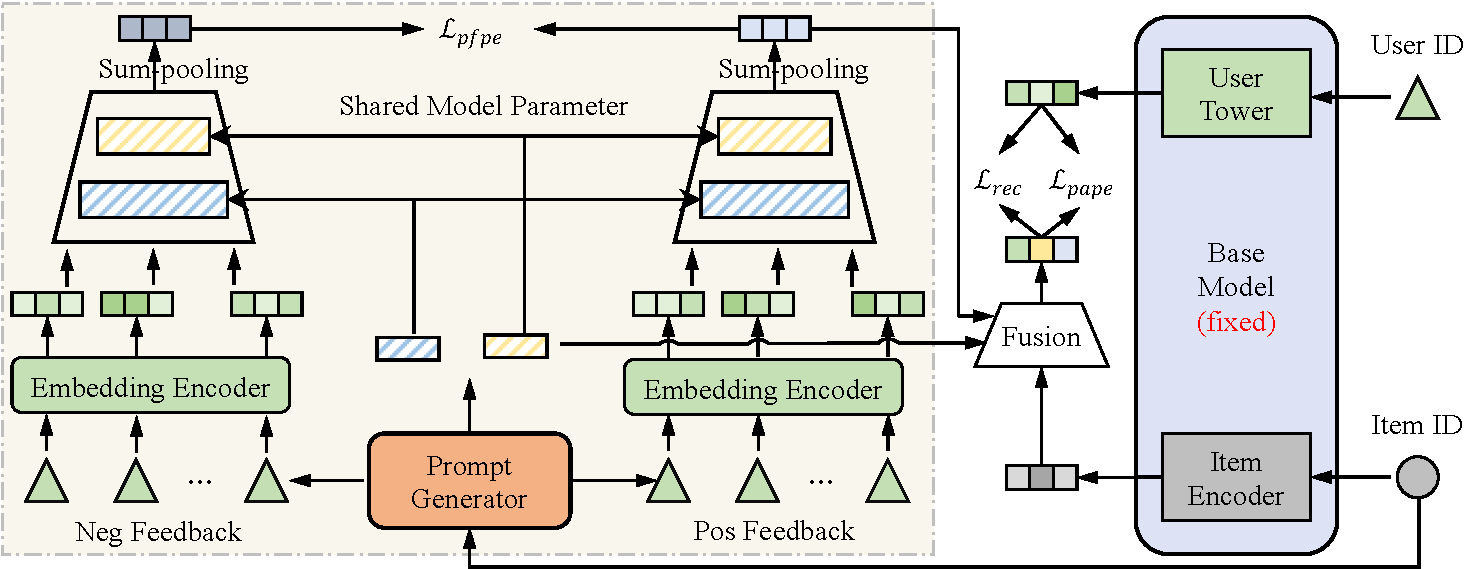
\includegraphics[width=1\linewidth]{figures/framework.pdf}
    \caption{Overview of our AtkPDM$^{+}$ algorithm: Starting from the leftmost latent of the initial adversarial image  $\mathbf{z}^{\adv}$, we first decode back to pixel-domain to perform forward diffusion with both $\mathbf{x}$ and $\mathbf{x}^{\adv}$ and feed them to frozen victim UNet. We then extract the feature representation in UNet to calculate our $\mathcal{L}_\text{attack}$, aiming to distract the recognition of image semantics. We also calculate our $\mathcal{L}_\text{fidelity}$ in pixel-domain to constrain the optimization. Finally, the $\mathbf{z}^{\adv}$ is being alternatively updated by loss gradients.}
    \label{framework}
\end{figure*}


\subsection{Overview}

To achieve effective protection against diffusion-based editing, we aim to push the protected sample away from the original clean sample by disrupting the intermediate step in the reverse diffusion process. For practical real-world applications, it's essential to ensure the protected image is perceptually similar to the original image. In practice, we uniformly sample the value of the forward diffusion step $t \sim [0, T]$ to generate noisy images and then perform optimization to craft the adversarial image $\mathbf{x}^{\adv}$ via our attacking and fidelity losses, repeating the same process $n$ times or until convergence. Figure \ref{concept} depicts these two push-and-pull criteria during different noise levels, the successful attack is reflected in the light orange line where the reverse sample moves far away from the normal edition of the image. More specifically, our method can be formulated as follows:

\begin{equation}
    \begin{aligned}
        & \max_{\mathbf{x}^{\adv} \in \mathcal{M}}
        \mathbb{E}_{
        t,
        \mathbf{x}_t| \mathbf{x}, \mathbf{x}_t^{\adv}| \mathbf{x}}
         \left[-\mathcal{L}_\text{attack}(\mathbf{x}_t, \mathbf{x}_t^{\adv})\right] \\
        & \text{subject to } \mathcal{L}_\text{fidelity}(\mathbf{x}, \mathbf{x}^{\adv}) \leq \delta,
    \end{aligned}
    \label{eq:probelm_setting_constraint}
\end{equation}

\noindent where $\delta$ denotes the attacking budget. The details of the attacking loss $\mathcal{L}_\text{attack}$ and the fidelity loss $\mathcal{L}_\text{fidelity}$ will be discussed in the following sections.


\subsubsection{Framework.}
Our framework is illustrated in Figure~\ref{framework}. We fix two identical victim UNets to extract feature representations of clean and protected samples for optimizing to push away from each other. A protection loss is jointly incorporated to constrain the optimization. After $N$ iterations, we segment out only the protecting main object of the image for better imperceptibility of image protection.

\subsection{Proposed Losses}
We propose two novel losses as optimization objectives to craft an adversarial example efficiently without running through all the diffusion steps. Attacking loss is designed to distract the feature representation in denoising UNet; Protection loss is a constraint to ensure the image quality. For notation simplicity, we first define the samples $\mathbf{x}, \mathbf{x}^{\adv}$ in different forwarded steps. 

Let $\mathcal{F}(\mathbf{x}, t, \epsilon) = \sqrt{\bar{\alpha}_t} \mathbf{x} + \sqrt{1-\bar{\alpha}_t} \epsilon$ be the diffusion forward process. Given timestep $t$ sample from $[0, T]$, noises $\epsilon_1, \epsilon_2$ sample from $\normaldist$. We denote $\mathbf{x}_t = \mathcal{F}(\mathbf{x}, t, \epsilon_1)$, and $\mathbf{x}^{\adv}_t = \mathcal{F}(\mathbf{x}^{\adv}, t, \epsilon_1)$.

\subsubsection{Attacking Loss.}
Our goal is to define effective criteria that could finally distract the reverse denoising process. PhotoGuard~\cite{salman2023raisingcostmaliciousaipowered} proposed to backpropagate through all the steps of the reverse denoising process via PGD, however, this approach is prohibitively expensive, Diff-Protect~\cite{xue2024effectiveprotectiondiffusionbased} proposed to avoid the massive cost by leveraging Score Distillation~\cite{poole2022dreamfusiontextto3dusing2d} in optimization. However, Diff-protect relies heavily on gradients of attacking encoder of an LDM as stated in their results. In PDM, we don't have such an encoder to attack; nevertheless, we find that the denoising UNet has a similar structure to encoder-decoder models, and some previous works~\cite{lin2024diffusionmodelperceptualloss, li2023fasterdiffusionrethinkingrole} characterize this property to accelerate and enhance the generation. From our observations of the feature roles in denoising UNets, we hypothesize that distracting specific inherent feature representation in UNet blocks could lead to effectively crafting an adversarial image. In practice, we first extract the feature representations of forwarded images $\mathbf{x}_t$ and $\mathbf{x}^{\adv}_t$ in frozen UNet blocks of timestep $t$. Then, we adopt 2-Wasserstein distance~\cite{arjovsky2017wasserstein} to measure the discrepancy in feature space. Note that we take the negative of the calculated distance, as we aim to pull the $\mathbf{x}^{\adv}_t$ away from $\mathbf{x}_t$. Formally, the attacking loss $\mathcal{L}_\text{attack}$ is defined as:
\begin{equation}
    \mathcal{L}_\text{attack}(\mathbf{x}_t, \mathbf{x}^{\adv}_t)
    =-\mathcal{W}_2 \left(
    \mathcal{U}^\text{(mid)}_{\theta}(\mathbf{x}_t), \mathcal{U}^\text{(mid)}_{\theta}(\mathbf{x}^{\adv}_t)
    \right).
\end{equation}

\noindent Assuming the feature distributions approximate Gaussian distributions expressed by mean $\mu_t$ and $\mu_t^{\adv}$, and non-singular covariance matrices $\Sigma_t$ and $\Sigma_t^{\adv}$. The calculation of the 2-Wasserstein distance between two normal distributions is viable through the closed-form solution~\cite{dowson1982frechet, olkin1982distance, chen2018optimal}:

\begin{equation}
    \begin{aligned}
        & \mathcal{W}_2^2(\mathcal{N}(\mu_t, \Sigma_t), \mathcal{N}(\mu_t^{\adv}, \Sigma_t^{\adv}))
        = \|\mu_t-\mu_t^{\adv}\|_2^2 \\
        & \qquad + \text{trace} (\Sigma_t + \Sigma_t^{\adv}
        -2({\Sigma_t^{\adv}}^{\frac{1}{2}}\Sigma_t{\Sigma_t^{\adv}}^{\frac{1}{2}})^\frac{1}{2} ).
    \end{aligned}
    \label{eq:wasserstein_distance}
\end{equation}

\subsubsection{Fidelity Loss.}
To control the attack budget for adversarial image quality, we design a constraint function that utilizes the feature extractor from a pretrained classifier for calculating fidelity loss. In our case, we sum up the 2-Wasserstein feature losses of $L$ different layers. Specifically, we define $\mathcal{L}_\text{fidelity}$ as:
\begin{equation}
    \mathcal{L}_\text{fidelity}(\mathbf{x}_t, \mathbf{x}^{\adv}_t)
    = \sum_{\ell=1}^L \mathcal{W}_2(\phi_\ell(\mathbf{x}), \phi_\ell(\mathbf{x}^{\adv})),
\end{equation}
where $\mathcal{W}_2$ denotes 2-Wasserstein distance and $\phi_\ell$ denotes layer $\ell$ of the feature extractor.


\subsection{Alternating Optimization for Adversarial Image}
We solve the constrained optimization problems via alternating optimization to craft the adversarial images, detailed optimization loop of AtkPDM$^{+}$ is provided in Algorithm ~\ref{alg:attdpmplus}. AtkPDM algorithm and the derivation of the alternating optimization are provided in Appendix.


\subsection{Latent Optimization via Pretrained-VAE}
Previous works suggest that diffusion models have a strong capability of resisting adversarial perturbations~\cite{xue2024pixelbarrierdiffusionmodels}, making them hard to attack via pixel-domain optimization. Moreover, they are even considered good purifiers of adversarial perturbations~\cite{nie2022diffusionmodelsadversarialpurification}. Here we propose a latent optimization strategy that crafts the ``perturbation'' in latent space. We adopt a pre-trained Variational Autoencoder (VAE) ~\cite{kingma2014autoencoding} to convert images to their latent space, and the gradients will be used to update the latent, after N iterations or losses converge, we decode back via decoder $\mathcal{D}$ to pixel domain as our final protected image. The motivation for adopting VAE is inspired by MPGD~\cite{he2024manifold}. This strategy is effective for crafting a robust adversarial image against pixel-domain diffusion models while also better preserving the protection quality rather than only incorporating fidelity constraints. The constraint optimization thereby becomes: 
\begin{equation}
\begin{aligned}
    & \max_{\mathbf{z}^{\adv}}
    \mathbb{E}_{
    t,
    \mathbf{x}_t| \mathbf{x}, \mathbf{x}_t^{\adv}| \mathcal{D}(\mathbf{z}^{\adv})}
    \left[-\mathcal{L}_\text{attack}(\mathbf{x}_t, \mathbf{x}_t^{\adv})\right] \\
    & \text{subject to } \mathcal{L}_\text{fidelity}(\mathbf{x}, \mathcal{D}(\mathbf{z}^{\adv})) \leq \delta.
\end{aligned}
\label{eq:probelm_setting_constraint}
\end{equation}

\noindent Detailed latent optimization loop is provided in Algorithm~\ref{alg:attdpmplus}.


\begin{algorithm}[t]
    \caption{AtkPDM$^{+}$}
    \label{alg:attdpmplus}
    \small{
    \begin{algorithmic}[1] 
        \STATE{\textbf{Input:}
        Image to be protected $\mathbf{x}$, attack budget $\delta > 0$, step size $\gamma_1, \gamma_2>0$, \textcolor{black}{VAE encoder $\mathcal{E}$, and VAE decoder $\mathcal{D}$}}
        \STATE{\textbf{Initialization:} $\mathbf{x}^{\adv} \leftarrow \mathbf{x}$, $L_\text{attack} \leftarrow \infty$}
        \STATE{\textcolor{black}{Encode adversarial image to latent space: $\mathbf{z}^{\adv} \leftarrow \mathcal{E}(\mathbf{x}^{\adv})$}}
        \WHILE{$L_\text{attack}$ not convergent}
            \STATE{\textcolor{black}{Decode adversarial latent to pixel space: $\mathbf{x}^{\adv} \leftarrow \mathcal{D}(\mathbf{z}^{\adv})$}}
            \STATE{Sample timestep: $t \sim [0, T]$}
            \STATE{Sample noise: $\epsilon_1, \epsilon_2 \sim \normaldist$}
            \STATE{Compute original noisy sample: $\mathbf{x}_t \leftarrow \mathcal{F}(\mathbf{x}, t, \epsilon_1)$}
            \STATE{Compute adversarial noisy sample: $\mathbf{x}^{\adv}_t \leftarrow \mathcal{F}(\mathbf{x}^{\adv}, t, \epsilon_2)$}
            \STATE{\textcolor{black}{Update $\mathbf{z}^{\adv}$ by Gradient Descent: \\
            $\mathbf{z}^{\adv} \leftarrow \mathbf{z}^{\adv} -
            \gamma_1 \sign(\nabla_{\mathbf{z}^{\adv}} \mathcal{L}_\text{attack}(\mathbf{x}_t, \mathbf{x}^{\adv}_t))$}}
            \WHILE{$\mathcal{L}_\text{fidelity}(\mathbf{x}, \textcolor{black}{\mathcal{D}(\mathbf{z}^{\adv})}) > \delta$}
            \STATE{ 
            \textcolor{black}{$\mathbf{z}^{\adv} \leftarrow \mathbf{z}^{\adv} -
            \gamma_2 \nabla_{\mathbf{z}^{\adv}} \mathcal{L}_\text{fidelity}(\mathbf{x}, \mathcal{D}(\mathbf{z}^{\adv}))$}}
            \ENDWHILE
        \ENDWHILE
        \STATE{\textcolor{black}{Decode adversarial latent to pixel space: $\mathbf{x}^{\adv} \leftarrow \mathcal{D}(\mathbf{z}^{\adv})$}}
        \RETURN {$\mathbf{x}^{\adv}$}
    \end{algorithmic}
    }
\end{algorithm}


\section{Experiment Results}
In this section, we examine the attack effectiveness and robustness of our approach under extensive settings. 


\begin{table}[tb]
    \centering
    \setlength{\tabcolsep}{1mm}
    \vspace{-2ex}
    \resizebox{1\columnwidth}{!}{
    \begin{tabular}{l|ccc|ccc}
    \toprule
        \multirow{2}{*}{Methods} &  \multicolumn{3}{@{}c}{{\bf GSM8K}} &  \multicolumn{3}{@{}c}{{\bf BBH}} \\
         & EM & Tokens & $1/\tau$ & EM & Tokens & $1/\tau$\\
        % \hline
         \cmidrule (r){1-1}\cmidrule (lr){2-4} \cmidrule (lr){5-7}
     Full-shot & 78.85 & 2,366 & - & 70.07 & 774 & -  \\
     \hline
     \hline
     \multicolumn{4}{@{}l}{{\bf \textit{1-shot constraint}}} \\ 
    1-shot & 77.10 & 422 & 6x & 69.60 & 284 & 3x \\
    Selective-Context & 53.98 & 452 & 5x & 54.27 & 276 & 3x \\
    GPT4 Generation & 71.87 & 496 & 5x & 27.13 & 260 & 3x \\
    {\cellcolor[rgb]{0.925,0.957,1}}\textbf{Ours} & {\cellcolor[rgb]{0.925,0.957,1}}\textbf{79.08} & {\cellcolor[rgb]{0.925,0.957,1}}446 & {\cellcolor[rgb]{0.925,0.957,1}}5x & {\cellcolor[rgb]{0.925,0.957,1}}\textbf{70.11} & {\cellcolor[rgb]{0.925,0.957,1}}288 & {\cellcolor[rgb]{0.925,0.957,1}}3x \\
     \hline
     \hline
     \multicolumn{4}{@{}l}{{\bf \textit{half-shot constraint}}} \\ 
    Sentence Selection & 72.33 & 230 & 10x & 39.56 & 175 & 4x\\
    Selective-Context & 52.99 & 218 & 11x & 54.02 & 155 & 5x \\
    GPT4 Generation & 68.61 & 223 & 11x & 27.09 & 161 & 5x \\
    {\cellcolor[rgb]{0.925,0.957,1}}\textbf{Ours} & {\cellcolor[rgb]{0.925,0.957,1}}\textbf{77.41} & {\cellcolor[rgb]{0.925,0.957,1}}171 & {\cellcolor[rgb]{0.925,0.957,1}}14x & {\cellcolor[rgb]{0.925,0.957,1}}\textbf{61.60} & {\cellcolor[rgb]{0.925,0.957,1}}171 & {\cellcolor[rgb]{0.925,0.957,1}}5x \\
     \hline
     \hline
     \multicolumn{4}{@{}l}{{\bf \textit{quarter-shot constraint}}} \\ 
    Sentence Selection & 66.67 & 195 & 12x & 46.00 & 109 & 7x \\
    Selective-Context & 44.20 & 157 & 15x & 47.37 & 108 & 7x \\
    GPT4 Generation & 56.33 & 188 & 20x & 26.81 & 101 & 8x \\
    {\cellcolor[rgb]{0.925,0.957,1}}\textbf{Ours} & {\cellcolor[rgb]{0.925,0.957,1}}\textbf{77.33} & {\cellcolor[rgb]{0.925,0.957,1}}117 & {\cellcolor[rgb]{0.925,0.957,1}}20x & {\cellcolor[rgb]{0.925,0.957,1}}\textbf{56.85} & {\cellcolor[rgb]{0.925,0.957,1}}110 & {\cellcolor[rgb]{0.925,0.957,1}}7x \\
     \hline
     \hline
    zero-shot & 48.75$^{\dag}$ & 11 & 215x & 32.32 & 16 & 48x \\
    Simple Prompt & 74.9 & 691 & 3x & - & - & - \\
    \bottomrule
    \end{tabular}
    }
    \caption{Performance of different methods under different target compression ratios on the GSM8K mathematical reasoning and Big-bench Hard (BBH) datasets. $^{\dag}$We also include the instruction of the prompt in zero-shot experiments for a vertical comparison.}
    \label{tab:main_results}
\end{table}



\begin{table}[t]
\footnotesize{
    \centering
    \begin{tabular}{lcccc}
        \toprule
        \multirow{2}{*}{Defense Method} & \multicolumn{4}{c}{Attacking Effectiveness} \\ 
         &  SSIM $\downarrow$ & PSNR $\downarrow$ & LPIPS $\uparrow$ & IA-Score $\downarrow$ \\
        \midrule
        Crop-and-Resize & 0.68 & 29.28 & 0.42 & 0.79 \\
        JPEG Comp. & 0.78  & 29.82 & 0.36 & 0.79 \\
        \midrule
        None & 0.79 & 30.05 & 0.33 & 0.81 \\
        \bottomrule
    \end{tabular}
    \caption{Quantitative results of our adversarial images against defense methods. Both Crop-and-Resize and JPEG Compression fail to defend our attack. ``None'' indicates no defense is applied, as the baseline for comparison.}
    % The term "None" in the defense method column indicates the use of the adversarial image generated by our method without applying any purification techniques.
\label{tab:defense}
}
\end{table}



\subsection{Experiment Settings}
\subsubsection{Implementation Details.} We conduct all our experiments in white box settings and examine the effectiveness of our attacks using SDEdit \cite{meng2021sdedit}. For the Variational Autoencoder (VAE) ~\cite{kingma2014autoencoding} in our AtkPDM$^{+}$, we utilize the VAE provided by StableDiffusion V1.5 ~\cite{rombach2022high}.
We run all of our experiments with 300 optimization steps, which is empirically determined, to balance attacking effectiveness and image protection quality with reasonable speed. Other loss parameters and running time are provided in the Appendix. The implementation is built on the Diffusers library. All the experiments are conducted with a single Nvidia Tesla V100 GPU.


\subsubsection{Victim Models and Datasets.}
We test our approach on PDMs with three open-source checkpoints on HuggingFace, specifically ``google/ddpm-ema-church-256'', ''google/ddpm-cat-256'' and ``google/ddpm-ema-celebahq-256''. For the results reported in Table~\ref{tab:attackPDM}, we run 30 images for each victim model. Additionally, for generalizability in practical scenarios, we synthesize the data with half randomly from the originally trained dataset and another half from randomly crawled with keywords from the Internet.

\subsubsection{Baseline Methods and Evaluation Metrics.}

To the best of our knowledge, previous methods have mainly focused on LDMs, and effective PDM attacks have not yet been developed, however, we still implement Projected Gradient Ascent (PGAscent) with their proposed semantic loss by~\cite{salman2023raisingcostmaliciousaipowered, liang2023adversarialexampledoesgood, liang2023mistimprovedadversarialexamples, xue2024effectiveprotectiondiffusionbased}. Notably, Diff-Protect~\cite{xue2024effectiveprotectiondiffusionbased} proposed to minimize the semantic loss is surprisingly better than maximizing the semantic loss, we also adopted this method in attacking PDMs and denote as Diff-Protect. To quantify the adversarial image visual quality, we adopted Structural Similarity (SSIM) ~\cite{wang2004image}, Peak Signal-to-Noise Ratio (PSNR), and Learned Perceptual Image Patch Similarity (LPIPS) ~\cite{zhang2018unreasonable}. We also inherit these three metrics, but negatively to quantify the effectiveness of our attack. We also adopted Image Alignment Score (IA-Score) \cite{kumari2023multi} that leverages CLIP \cite{radford2021learning} to calculate the cosine similarity of image encoder features. In distinguishing from previous methods, to more faithfully reflect the attack effectiveness, we fix the same seed of the random generator when generating clean and adversarial samples, then calculate the scores based on the paired samples.

\subsection{Attack Effectiveness on PDMs}

As quantitatively reported in Table~\ref{tab:attackPDM} and qualitative results in Figure~\ref{qualitative}, compared to previous PGD-based methods incorporating semantic loss, i.e., negative training loss of diffusion models, our method exhibits superior performance in both adversarial image quality and attacking effectiveness. And our reported figures has generally stable as reflected in lower standard deviation. It is worth noting that even if the adversarial image qualities of the PGD-based methods are far worse than ours, their attacking effectiveness still falls short, suggesting that PDMs are robust against traditional perturbation methods, this finding is also aligned with previous works~\cite{xue2024effectiveprotectiondiffusionbased,xue2024pixelbarrierdiffusionmodels}. For AtkPDM$^+$, combined with our latent optimization strategy, the adversarial image quality has enhanced while slightly affecting the attacking effectiveness, still outperforming the previous methods.



\begin{table}[t]
\footnotesize{
    \centering
    \begin{tabular}{lcccc}
        \toprule
        \multirow{2}{*}{Setting} & \multicolumn{4}{c}{Attacking Effectiveness} \\ 
         &  SSIM $\downarrow$ & PSNR $\downarrow$ & LPIPS $\uparrow$ & IA-Score $\downarrow$ \\
        \midrule
        White Box & 0.79 & 30.05 & 0.33 & 0.81 \\
        
        Black Box & 0.86 & 30.25 & 0.29 & 0.85 \\
    
        \midrule
        Difference & 0.07 & 0.20 & 0.04 & 0.04 \\
        \bottomrule
    \end{tabular}
    \caption{Quantitative results of black box attack. We use the same set of adversarial images and feed to white box and black box models to examine the black box transferability.} 
\label{tab:blackBox}
}
\end{table}
\begin{figure*}[t]
\centering
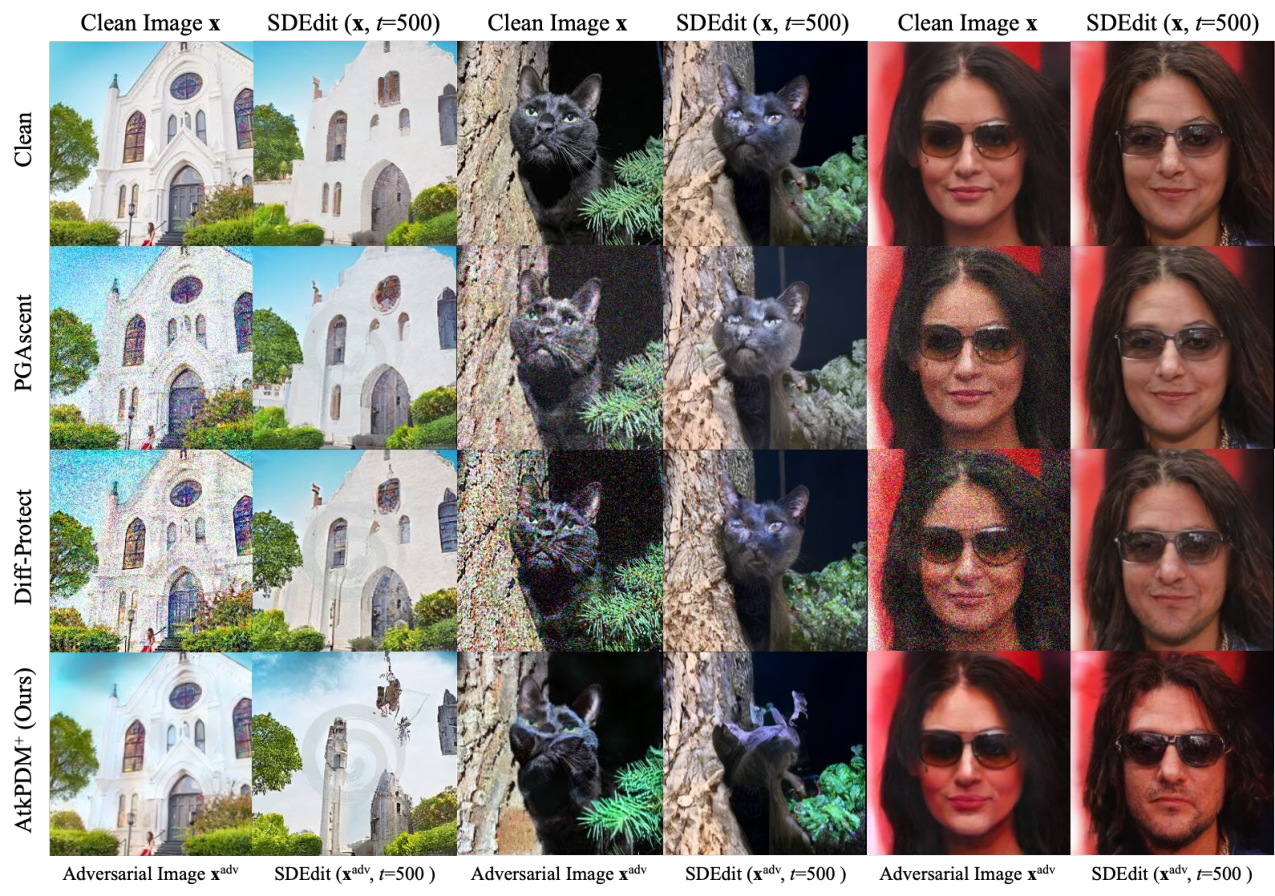
\includegraphics[width=0.79\linewidth]{figures/qualitative_results.pdf}
\caption{Qualitative results compared to previous methods: our adversarial images can effectively corrupt the edited results without significant fidelity decrease. The same column shares the same random seed for fair comparison.
}
\label{qualitative}
\end{figure*}

\begin{table*}
    \centering
    \small{
    \begin{tabular}{lc|ccc|cccc}
        \toprule
        \multirow{2}{*}{Losses} & \multirow{2}{*}{VAE} & \multicolumn{3}{c|}{Adversarial Image Quality} & \multicolumn{4}{c}{Attacking Effectiveness} \\ 
         & & SSIM $\uparrow$ & PSNR $\uparrow$ & LPIPS $\downarrow$ & SSIM $\downarrow$ & PSNR $\downarrow$ & LPIPS $\uparrow$ & IA-Score $\downarrow$ \\
        \midrule
        $\mathcal{L}_\text{semantic}$ &  & 0.37 $\pm$ 0.09  & 28.17 $\pm$ 0.22 & 0.73 $\pm$ 0.16  & 0.89 $\pm$ 0.05 & 31.06 $\pm$ 1.94 & 0.17 $\pm$ 0.09 & 0.93 $\pm$ 0.04 \\
        $\mathcal{L}_\text{semantic}$ & \checkmark & 0.80 $\pm$ 0.05 & \second{29.78} $\pm$ 0.42 & \second{0.17} $\pm$ 0.03 & 0.82 $\pm$ 0.05 & 30.43 $\pm$ 0.75 & 0.15 $\pm$ 0.06 & 0.92 $\pm$ 0.04 \\
        % $\mathcal{L}_\text{semantic}$ + $\mathcal{L}_\text{fidelity}$ &  & 0.12  & 27.90 & 1.08 & \first{0.58} & \first{28.01} & \first{0.93} & \first{0.61} \\ 
        $\mathcal{L}_\text{semantic}$ + $\mathcal{L}_\text{fidelity}$ & \checkmark & \first{0.82} $\pm$ 0.05 & \first{30.30} $\pm$ 0.81 & \first{0.13} $\pm$ 0.03 & 0.90 $\pm$ 0.03 & 31.24 $\pm$ 1.19 & 0.08 $\pm$ 0.03 & 0.96 $\pm$ 0.02 \\
        \midrule
        $\mathcal{L}_\text{attack}$ + $\mathcal{L}_\text{fidelity}$ (Ours) & & 0.75 $\pm$ 0.03 & 28.22 $\pm$ 0.10  & 0.26 $\pm$ 0.04 & \first{0.75} $\pm$ 0.04 & \first{29.61} $\pm$ 0.23 & \first{0.40} $\pm$ 0.05 & \first{0.76} $\pm$ 0.06 \\
        $\mathcal{L}_\text{attack}$ + $\mathcal{L}_\text{fidelity}$ (Ours) & \checkmark & \second{0.81} $\pm$ 0.03 & 28.64 $\pm$ 0.19 & \first{0.13} $\pm$ 0.02 & \second{0.79} $\pm$ 0.04 & \second{30.05} $\pm$ 0.47 & \second{0.33} $\pm$ 0.07 & \second{0.81} $\pm$ 0.06 \\
        \bottomrule
    \end{tabular}
    }
    \caption{Quantitative results of ablation study. The best is in bold and the second best is underlined. Errors denote one standard deviation of all images in our test datasets.}
    \label{tab:loss_ablation}
    \vspace*{-10pt}
\end{table*}



\subsection{Against Defense Methods}
We examine the robustness of our approach against two widely recognized and effective defense methods for defending against adversarial attacks as reported in Table~\ref{tab:defense}.

\subsubsection{Crop and Resize.}
Noted by Diff-Protect, crop and resize is simple yet the most effective defense method against their attacks on LDMs. We also test our method against this defense using their settings, i.e., cropping 20\% of the adversarial image and then resizing it to its original dimensions.


\subsubsection{JPEG Compression.}
Sandoval-Segura et al.~\cite{sandoval2023jpeg} demonstrated that JPEG compression is a simple yet effective adversarial defense method. In our experiments, we implement the JPEG compression at a quality setting of 25\%. The quantitative results in Table~\ref{tab:defense} demonstrate that our method is robust against these two defense methods, with four of the metrics listed in Table~\ref{tab:defense} are not worse than no defenses. Surprisingly, these defense methods even make the adversarial image more effective than cases without defense.


\subsection{Black Box Transferability}
We craft adversarial images with the proxy model, ``google/ddpm-ema-church-256'', in white-box settings and test their transferability to another ``google/ddpm-bedroom-256'' model for black-box attacks. Under identical validation settings, Table~\ref{tab:blackBox} reveals only a slight decrease in attack effectiveness metrics, indicating successful black-box transferability.



\subsection{Effectiveness of Latent Optimization via VAE}
We first incorporate our VAE latent optimization strategy in the previous semantic-loss-based PGAscent. From Table~\ref{tab:loss_ablation}, without using $\mathcal{L}_\text{fidelity}$, latent optimization has significantly enhanced the adversarial image quality and even slightly improved the attacking effectiveness. Adopting latent optimization in our approach enhances visual quality with a negligible decrease in attacking effectiveness. Surprisingly, incorporating our $\mathcal{L}_\text{fidelity}$ with current PGD-based method will drastically decrease the adversarial image quality despite its attack performing better than ours. This may be due to different constrained optimization problem settings.

\section{Discussion}
% \subsection{Concurrent Work}
% In recent years it has become more popular to release ``uncensored'' language models, and with that there have been tools and techniques developed to detect undesirable outputs produced by these models. One such tool is Llama Guard \cite{inan2023llama}, a large language model designed to perform both prompt- and response-classification to maximise the safety of chat systems. Like DPH, Llama Guard can be used to detect and reject harmful outputs produced by a language model. However, unlike DPH, Llama Guard is an entirely separate model which must be run concurrently with chat model and therefor increases the compute and memory requirements of the combined system. % this especially contrasts with DPH being especially suited for small language models which inherently require a much smaller compute budget.

\subsection{Future Work}
As shown in the results section, DPH is capable of learning to assign higher rewards to preferred outputs and lower rewards to dispreferred outputs which implies the pooling function learns rich features with respect to prompt-completion pairs. We believe that it would be possible to also extract additional information from the output of the pooling function to detect finer grained signals such as helpfulness, humor, creativity, toxic content, etc. This can be achieved by training on a conversational dataset such Open Assistant \cite{köpf2023openassistant} which contains a variety of human-curated labels in addition to machine-generated labels produced by Detoxify \cite{Detoxify}.

% It is also worth examining how the performance of DPH scales with larger language models, and if it can be used as a post-hoc technique to provide safety guardrails for uncensored language models such as Mistral 7B and observe how it performs compared to systems such as Llama Guard while maintaining much lower compute requirements.

\subsection{Limitations}
The main benefit of DPH being its ability to perform alignment without directly effecting the model's output distribution is also its main limitation: unlike other alignment techniques which can help prevent the model generating harmful outputs, DPH is only capable of \textit{detecting} harmful outputs. Although we do include DPO alignment in our experiments to reduce the likelihood of harmful outputs, DPH does not require such model alignment to function, which shifts the responsibility of rejecting harmful outputs to the end user or service provider.

\subsection{Conclusion}
In this paper we introduced Direct Preference Heads, a novel form of language model alignment which is performed at inference time to prune candidate completions for a given prompt. Unlike other alignment techniques which coerce the model into generating human preference aligned outputs, DPH instead produces reward scores for candidate outputs without affecting the actual generation process and therefor avoids the issue of RLHF leading to degraded performance when applied to smaller language models. We formulated two loss functions for DPH and find strong connections to Conservative DPO, implying that DPH is robust to label noise and can be tuned to a specific confidence margin. Finally, we evaluated our methods on a number of NLU, commonsense reasoning and reading Comprehension tasks and found that DPH is able to consistently outperform both our SFT baseline and multiple publicly available language model checkpoints of varying size and training volume.

\subsection*{Broader Impacts}
As with all language modeling systems we cannot guarantee all responses produced by our models are factually correct nor can we guarantee that they are safe and free from harmful content. Our work focuses on creating a system that helps filter out incorrect and harmful messages by scoring candidate outputs, but as with all alignment techniques our models may be susceptible to so-called `jailbreaks' which can coerce the model into incorrectly assigning a higher score to less desirable content. To maximise safety DPH should be implemented alongside other safety guardrails such as Llama Guard \cite{inan2023llama} when used for publicly facing chat systems, and we intend for our provided model checkpoints to be used for reproduction of results and further research in the field of alignment.

{
    \small
    \bibliographystyle{ieeenat_fullname}
    \bibliography{main}
}

% WARNING: do not forget to delete the supplementary pages from your submission 
\clearpage
\setcounter{page}{1}
\maketitlesupplementary


\section{Rationale}
\label{sec:rationale}
% 
Having the supplementary compiled together with the main paper means that:
% 
\begin{itemize}
\item The supplementary can back-reference sections of the main paper, for example, we can refer to \cref{sec:intro};
\item The main paper can forward reference sub-sections within the supplementary explicitly (e.g. referring to a particular experiment); 
\item When submitted to arXiv, the supplementary will already included at the end of the paper.
\end{itemize}
% 
To split the supplementary pages from the main paper, you can use \href{https://support.apple.com/en-ca/guide/preview/prvw11793/mac#:~:text=Delete%20a%20page%20from%20a,or%20choose%20Edit%20%3E%20Delete).}{Preview (on macOS)}, \href{https://www.adobe.com/acrobat/how-to/delete-pages-from-pdf.html#:~:text=Choose%20%E2%80%9CTools%E2%80%9D%20%3E%20%E2%80%9COrganize,or%20pages%20from%20the%20file.}{Adobe Acrobat} (on all OSs), as well as \href{https://superuser.com/questions/517986/is-it-possible-to-delete-some-pages-of-a-pdf-document}{command line tools}.

\end{document}
